\documentclass[10pt,a4paper]{report}
\usepackage[utf8]{inputenc}
\usepackage[russian]{babel}
\usepackage[OT1]{fontenc}
\usepackage{amsmath}
\usepackage{amsfonts}
\usepackage{amssymb}
\usepackage{graphicx}
\begin{document}
\title{Описание протокола}
\begin{enumerate}
\item При запуске сервера выводится сообщение, просящее ввести имя пользователя и пароль. Процедура повторяется пока пользователь не введет корректную пару логин/пароль. Пользователь может завершить сеанс командой exit.
\item При авторизации пользователя на экран выводятся еще не прочитанные им посты
\item При введении команды posts выводится структура форума
\item При введении команды show id_post выводится сообщение форума
\item При введении команды online выводится список активных пользователей
\item При введении команды add пользователю предлагается ввести имя темы, название поста и сообщение поста, после чего сообщение будет добавлено новое сообщение
\end{enumerate}
Ниже представлена sequence - диаграмма работы клиента - сервера
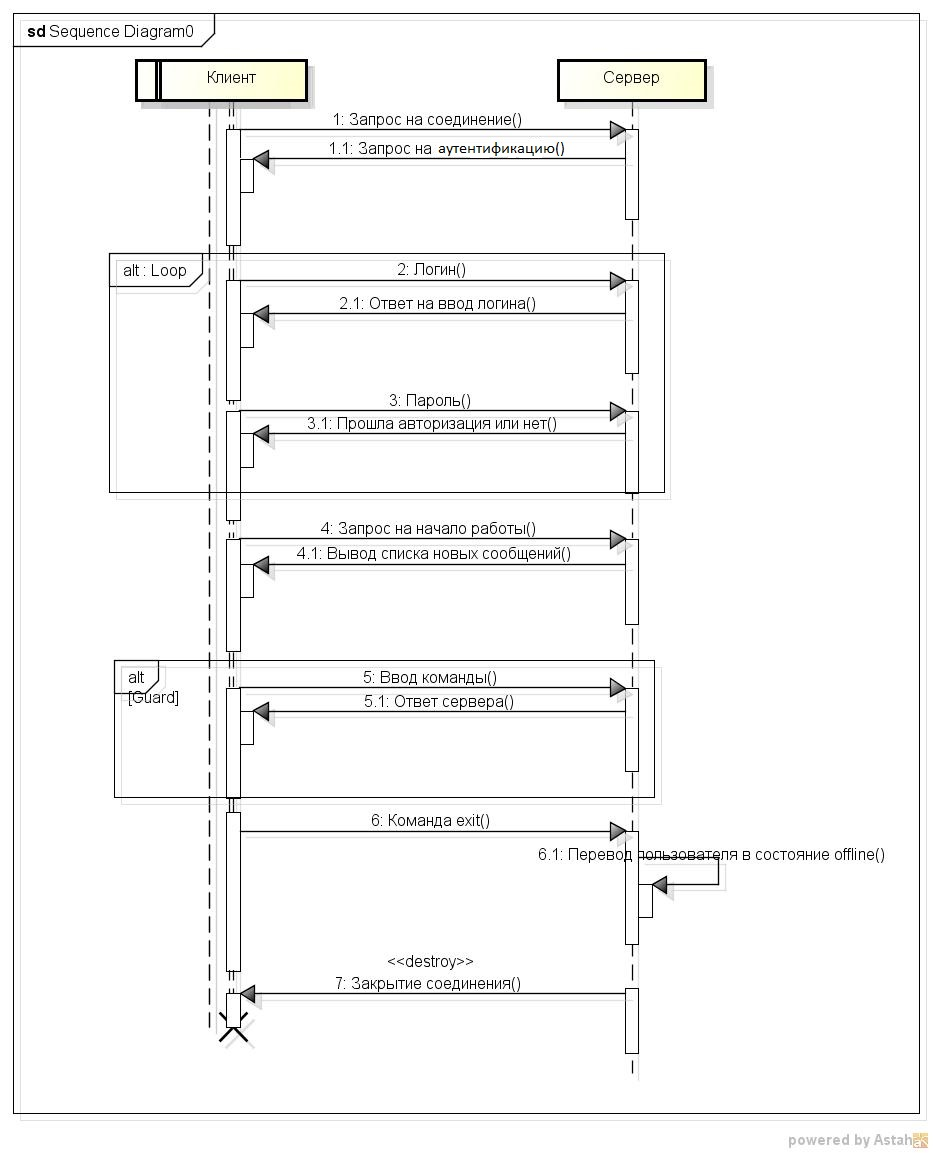
\includegraphics[scale=0.9]{diagram}
\end{document}